%==============================================================================
% Sjabloon onderzoeksvoorstel bachproef
%==============================================================================
% Gebaseerd op document class `hogent-article'
% zie <https://github.com/HoGentTIN/latex-hogent-article>

% Voor een voorstel in het Engels: voeg de documentclass-optie [english] toe.
% Let op: kan enkel na toestemming van de bachelorproefcoördinator!
\documentclass{hogent-article}

% Invoegen bibliografiebestand
\addbibresource{voorstel.bib}

% Informatie over de opleiding, het vak en soort opdracht
\studyprogramme{Professionele bachelor toegepaste informatica}
\course{Bachelorproef}
\assignmenttype{Onderzoeksvoorstel}
% Voor een voorstel in het Engels, haal de volgende 3 regels uit commentaar
% \studyprogramme{Bachelor of applied information technology}
% \course{Bachelor thesis}
% \assignmenttype{Research proposal}

\academicyear{2023-2024} % TODO: pas het academiejaar aan

% TODO: Werktitel
\title{Vul hier de voorgestelde titel van je onderzoek in}

% TODO: Studentnaam en emailadres invullen
\author{Ernst Aarden}
\email{ernst.aarden@student.hogent.be}

% TODO: Medestudent
% Gaat het om een bachelorproef in samenwerking met een student in een andere
% opleiding? Geef dan de naam en emailadres hier
% \author{Yasmine Alaoui (naam opleiding)}
% \email{yasmine.alaoui@student.hogent.be}

% TODO: Geef de co-promotor op
\supervisor[Co-promotor]{S. Beekman (Synalco, \href{mailto:sigrid.beekman@synalco.be}{sigrid.beekman@synalco.be})}

% Binnen welke specialisatierichting uit 3TI situeert dit onderzoek zich?
% Kies uit deze lijst:
%
% - Mobile \& Enterprise development
% - AI \& Data Engineering
% - Functional \& Business Analysis
% - System \& Network Administrator
% - Mainframe Expert
% - Als het onderzoek niet past binnen een van deze domeinen specifieer je deze
%   zelf
%
\specialisation{Mobile \& Enterprise development}
\keywords{Scheme, World Wide Web, $\lambda$-calculus}

\begin{document}

\begin{abstract}
  Hier schrijf je de samenvatting van je voorstel, als een doorlopende tekst van één paragraaf. Let op: dit is geen inleiding, maar een samenvattende tekst van heel je voorstel met inleiding (voorstelling, kaderen thema), probleemstelling en centrale onderzoeksvraag, onderzoeksdoelstelling (wat zie je als het concrete resultaat van je bachelorproef?), voorgestelde methodologie, verwachte resultaten en meerwaarde van dit onderzoek (wat heeft de doelgroep aan het resultaat?).
\end{abstract}

\tableofcontents

% De hoofdtekst van het voorstel zit in een apart bestand, zodat het makkelijk
% kan opgenomen worden in de bijlagen van de bachelorproef zelf.
%---------- Inleiding ---------------------------------------------------------

\section{Introductie}%
\label{sec:introductie}

Vele bedrijven zoeken tegenwoordig naar automatisering om competitief te blijven en repetitieve en nadeloze taken uit te sluiten. 
Zeker in IT-bedrijven is dit cruciaal om steeds onderzoek te doen naar nieuwe en betere oplossingen, dat is bij Aware niet anders. 
Aware zoekt momenteel naar manieren om nieuwe klanten makkelijker en vooral sneller op te zetten, om security redenen 
moeten deze klanten op aparte instanties opgezet worden. In dit onderzoek wordt gekeken 
aan de hand van een Proof of Concept of een automatiseringstool met name Ansible een mogelijke oplossing zou kunnen bieden 
om instanties op AWS Lightsail te configureren. De resultaten kunnen bijdragen aan de 
verdere ontwikkeling van dit concept of juist aanwijzen dat dit geen haalbare mogelijkheid is.

%---------- Stand van zaken ---------------------------------------------------

\section{State-of-the-art}%
\label{sec:state-of-the-art}

\subsection{Wat is Ansbile?}
\label{subsec:Wat is Ansible?}
Ansible is een open-source automatiseringsplatform dat kan worden gebruikt om grote groepen computersystemen te beheren. 
Het helpt je bij het automatiseren van de implementatie van applicaties, configuratiebeheer, cloud provisioning, 
het updaten van werkstations en servers en vele andere taken. 
\par 
Ansible werkt op Windows en Unix systemen en is opgenomen 
als onderdeel van de Fedora distributie. Maar machines die gebruikt worden om de automatisering uit te voeren - 
controleknooppunten genoemd - moeten Unix/Linux systemen zijn. Je kunt Windows machines gebruiken, 
maar met een Windows Subsystem for Linux distributie. 
\par
Een van de meest opwindende aspecten van Ansible is dat het zonder 
agents werkt, in tegenstelling tot de meeste andere oplossingen voor configuratiebeheer. 
Het vereist geen systemen op afstand met een specifieke agent of software om wijzigingen 
aan te brengen of opdrachten uit te voeren
\autocite{Manjaly2022}.

\subsection{Voordelen van Ansible}
\label{Voordelen van Ansible}

\begin{enumerate}
  \item Het vermindert de middelen die nodig zijn voor IT-beheer - Sysadmins kunnen honderden of zelfs duizenden machines 
  vanaf één punt en in één keer beheren.

  \item Het maakt automatisering toegankelijk - Een van de ontwerpdoelen van Ansible was dat er minimale kennis nodig zou zijn 
  om het te gebruiken. Het platform gebruikt YAML (Yet Another Markup Language), een voor mensen leesbare taal met elementen 
  uit andere gangbare programmeertalen.

  \item Het Ansible platform heeft geen invloed op de prestaties - Ansible vereist geen agents of software die op beheerde 
  systemen draait of geïnstalleerd is. Daarom hoeven beheerde systemen geen rekenkracht aan Ansible te besteden.

  \item Het zorgt voor consistentie - Het platform is ontworpen om minimaal te zijn en gebruikers in staat te stellen consistente 
  omgevingen te creëren. En de hele operatie verloopt via een SSH-verbinding, wat betekent dat het forum niet nog meer 
  complexiteit toevoegt aan de systemen
  \autocite{Manjaly2022}.
\end{enumerate}
%   \subsection{Hoe werkt Ansible?}
% \label{Hoe werkt Ansible?}
% Ansible werkt door 'Modules' of code uit te voeren op doelmachines die beheerde knooppunten worden genoemd. 
% Modules worden na uitvoering verwijderd van de doelsystemen. Deze modules kunnen van alles zijn, 
% van het kopiëren van een bestand naar een externe machine en het maken van een gecomprimeerd archief van bestanden tot 
% het beheren van VLAN-interfaces.
% \par
% In Ansible is een Task een eenvoudige actie die wordt toegepast op doelmachines. 
% Taken gebruiken Modules om een actie uit te voeren op een apparaat op afstand. 
% Deze Taken worden verder gerold in een geordende lijst in een Play. Een Play definieert welke taken worden toegepast op 
% welke machines.
% \par
% Alle Plays worden gecombineerd tot een zogenaamd Playbook. Dit is waar gebruikers alle Ansible-code schrijven. 
% Het Ansible playbook wordt uitgevoerd op een controleknooppunt en de Plays worden uitgevoerd in de volgorde waarin het is
% geschreven. De Taken binnen de Plays worden op hun beurt op dezelfde manier uitgevoerd. Wanneer een Taak wordt uitgevoerd, 
% stuurt het controleknooppunt de respectievelijke Modules naar alle doelmachines (beheerde knooppunten) die aan de taak zijn 
% gekoppeld. Ansible Modules of, op hun beurt, Ansible Playbooks zijn over het algemeen idempotent. 
% Dit betekent dat voordat de module wordt uitgevoerd, wordt gecontroleerd of het beheerde knooppunt al de gewenste status heeft. 
% Zo ja, dan wordt daar geen actie uitgevoerd
% \autocite{Manjaly2022}.

\subsection{Wat is AWS Lightsail?}
\label{Wat is AWS Lightsail?}
Amazon Lightsail is een AWS dienst die virtual private server (VPS) instances, containers, opslag en beheerde databases biedt 
tegen een kosteneffectieve en voorspelbare maandelijkse prijs. Het is bedoeld als de eenvoudigste manier om aan de slag te 
gaan met AWS voor kleine bedrijven, studenten, ontwikkelaars en anderen die hun website of applicaties voor algemene doeleinden 
in de cloud willen hosten.
\par
Lightsail is ontworpen met eenvoud in het achterhoofd, waardoor het gemakkelijk is voor gebruikers om websites en 
applicaties te implementeren die misschien niet veel cloudervaring hebben. De eenvoudige interface biedt gebruikers een 
minimaal aantal opties om te configureren, zodat ze hun bronnen snel en betrouwbaar kunnen inzetten zonder extra kennis of 
AWS-ervaring
\autocite{Graf2022}.

\subsection{Waarom kiezen voor AWS?}
\label{Waarom kiezen voor AWS?}
Je betaalt geen extra kosten voor de manier waarop de infrastructuur is aangeschaft en gelicentieerd, 
en zodra je deze diensten niet meer gebruikt, schakel je het uit en betaal je er niet meer voor.
Hoewel er een aantal grote spelers op de markt zijn, waaronder Azure (Microsoft), Google Cloud, IBM Cloud en Oracle, 
was AWS op het moment van schrijven nog steeds de belangrijkste speler in de ruimte
\autocite{Sesto2022}.

\subsection{Waarom Ansible voor cloud automation?}
\label{Waarom Ansible voor cloud automation?}
Cloud provisioning is een cruciaal onderdeel van het moderne cloud computing-model. 
We leven in het tijdperk van microservices, waar automatisering geen nice-to-have meer is. 
Het is een integraal onderdeel geworden van de dagelijkse activiteiten.
\par
Gelukkig is er een grote verscheidenheid aan automatiserings- en orkestratietools. 
Deze tools kunnen ons tijd besparen en tegelijkertijd de prestaties en nauwkeurigheid van provisionerings- en 
configuratiebeheerprocessen verbeteren.
\par
Ansible is in de eerste plaats een automatiseringstool. Met de juiste inhoud (rollen, modules en andere plugins) kan Ansible bijna 
alles automatiseren. En cloudbeheer is geen uitzondering, wat betekent dat we onze provisioneringsprocessen met relatief gemak 
kunnen automatiseren.
\par
Met een beetje hulp van producten voor continue integratie en continue implementatie (CI/CD) kan Ansible veranderen in een 
machtige orkestratietool. We kunnen beginnen met het combineren van op zichzelf staande taken tot complexe workflows die 
complexe IT-processen automatiseren.
\par
En als we workflowuitvoeringen koppelen aan gebeurtenissen uit onze monitoringsystemen, 
hebben we een aantal serieuze stappen gezet in de richting van een zelfherstellende infrastructuur
\autocite{Borovšak2021}.

% Voor literatuurverwijzingen zijn er twee belangrijke commando's:
% \autocite{KEY} => (Auteur, jaartal) Gebruik dit als de naam van de auteur
%   geen onderdeel is van de zin.
% \textcite{KEY} => Auteur (jaartal)  Gebruik dit als de auteursnaam wel een
%   functie heeft in de zin (bv. ``Uit onderzoek door Doll & Hill (1954) bleek
%   ...'')

% Je mag deze sectie nog verder onderverdelen in subsecties als dit de structuur van de tekst kan verduidelijken.

%---------- Methodologie ------------------------------------------------------
\section{Methodologie}%
\label{sec:methodologie}

Aan de hand van een Proof of Concept zal er uitgemaakt worden of dit onderzoek bruikbaar is voor Aware en of er aan de benodigde 
vereisten voldaan wordt, zoals schaalbaarheid, eenvoud en tijdswinst. De gehele opstelling zal op een Github-repository staan, zodat 
deze eenvoudig te repliceren is.

\subsection{Fase 1: Literatuurstudie}
\label{subsec:Fase 1: Literatuurstudie}
Wetenschappelijke artikels en boeken worden geraadpleegd op platformen zoals Google Scholar en Springer om 
kennis over het onderwerp op te doen. 
Andere onderzoeken moeten niet noodzakelijk voor corresponderende doeleinden zijn om ons een beter perspectief geven op dit onderzoek. 
Bestaande methodes en technieken zullen geanalyseerd worden en bijgehouden worden in een document om de meest effectieve aanpak te zoeken.
Deze fase loopt parallel met de volgende fasen tot er een conclusie is gevormd, dit zal naar schatting 10 weken aanhouden.

\subsection{Fase 2: Architectuurplan maken}
\label{subsec:Fase 2: Architectuurplan maken}
Van zodra er een idee is van hoe en wat, kan er een architectuurplan gemaakt worden waarmee het onderzoek uitgevoerd zal worden. 
Het architectuurplan zal bestaan uit onder andere de virtuele machines met hun virtuele hardware, tools die gebruikt worden om 
het onderzoek te realiseren en het gekozen besturingssysteem, in dit geval is dat Ubuntu.
Daarnaast zal ook de benodigde SaaS (Software as a Service) die moet draaien op de virtuele machine en een lijst van zowel functionele eisen 
(bv. use cases en vereisten) als niet-functonele eisen (bv. beveiliging en schaalbaarheid) in het architectuurplan inbegrepen zijn. 
De geschatte tijdsduur voor deze fase bedraagt 2 weken.

\subsection{Fase 3: Cloudomgeving opzetten met Ansible}
\label{subsec:Fase 3: Cloudomgeving opzetten met Ansible}
Aan de start van deze fase wordt er een AWS Account aangemaakt. Via een Bash-script is het mogelijk om eenvoudig nieuwe AWS Lightsail 
instanties aan te maken met de bijhorende specificaties, De nieuwe VPS (Virtual Private Server) zal direct weggeschreven worden 
naar het inventaris bestand zodat het playbook later kan gerunt worden met de VPS als doel. 
Om dit Bash-script te runnen wordt er gebruik gemaakt van WSL (Windows Subsystem for Linux). WSL zorgt ervoor dat Bash-scripts kunnen 
runnen op een Windows toestel (het controle knooppunt), een alternatief is om een virtuele machine te maken met Linux als OS. Om ervoor te zorgen 
dat dit script ook werkt, wordt AWS CLI geïnstalleerd en geconfigureerd (Access Key ID en Secret Access Key), 
zonder dit kunnen er geen nieuwe AWS Lightsail instanties aangemaakt worden. 
In deze fase wordt er een eerste instantie gecreëerd die de specificaties bevat uit het architectuurplan, deze eerste VPS 
zal in de volgende fase de benodigde configuraties krijgen. Hiervoor worden 3 weken ingepland.

\subsection{Fase 4: Playbook maken}
\label{subsec:Fase 4: Playbook maken}
De volgende uitdaging is het maken van het playbook, hierbij worden allerlei taken gedefinieerd zoals bv. het Installeren van 
software en enkele configuraties. De software die geïnstalleerd moet worden is PimLayer, PIM staat voor Product Information 
Management en dient om een bedrijf te helpen met grote hoeveelheid complexe productinformatie. 
AWS Lightsail gaat standaard zelf enkele basisconiguraties voor het netwerk en voor beveiliging 
voor ons uitvoeren. Dit zorgt er dus voor dat deze fase al wat lichter wordt. Na deze fase, die naar schatting 
3 weken duurt, is er een werkend en herbruikbaar playbook. 

\subsection{Fase 5: Testen}
\label{subsec:Fase 5: Testen}
Deze fase wordt tijdens fase 2 en 3 continue toegepast, door agile te werken wordt het script telkens uitgebreid en krijgt het playbook 
telkens nieuwe functionaliteiten. Dit wordt gedaan tot het bash-script succesvol is 
en het playbook foutloos is en doet wat er van verwacht wordt. Testen van het playbook is in feite vrij eenvoudig, doordat dit idempotent is 
kan dit zoveel worden uitgevoerd naar wens. Op het moment dat de vorige testen succesvol waren, kan er overgegaan worden naar het testen 
van de eenvoud om nieuwe instanties te lanceren. Deze test zou moeten nabootsen hoe het er in een echte situatie aan toe zou kunnen gaan. 
Om deze test uit te voeren, wordt het bestaande Bash-script opnieuw uitgevoerd. Vervolgens wordt het playbook gerunt en zou de nieuwe instantie 
in principe klaar moeten zijn voor gebruik. Omdat sommige klanten verschillende noden kunnen hebben, wordt deze instantie lichtelijk anders geconfigureerd. 
Dit kan bv. met de grootte van de instantie en de manier waarop de SaaS geconfigureerd wordt. Om een vergelijkingspunt te creëren, zal er opnieuw 
een instantie worden aangemaakt, maar deze keer zal dit handmatig gebeuren, zonder gebruik te maken van Ansible. 
De tijdsduur van deze fase wordt geschat op 8 weken, 6 weken tijdens fase 2 en 3, plus twee een extra week voor het 
aanmaken van de nieuwe instanties.

\subsection{Fase 6: Rapporteren}
\label{subsec:Fase 6: Rapporteren}
Na de testfase wordt een rapport opgesteld waarin wordt beoordeeld in welke maten het Proof of Concept een oplossing bied en 
een antwoord geeft aan de onderzoeksvraag. Doordat er zowel manueel als geautomatiseerd instanties kunnen worden opgezet, kunnen 
factoren zoals eenvoud en snelheid vergeleken worden. Hiervoor wordt er gerekend op 
een week tijd

\subsection{Fase 7: Regelmatige \\feedback-momenten houden}
\label{subsec:Fase 7: Regelmatige feedback-momenten houden}
Het regelmatig afspreken met de co-promoter is essentieel om feedback en kritiek te ontvangen, te onderzoeken en om te verbeteren en 
uiteindelijk te realiseren. Deze momenten worden doorheen het volledige onderzoek gehouden.

\subsection{Fase 8: Conclusie}
\label{subsec:Fase 8: Conclusie}
Uit het rapport kan het antwoord op de onderzoeksvraag afgeleid worden. In deze fase kunnen er 
mogelijks zowel positieve zaken als negatieve zaken aangekaart worden. Er wordt een week voorzien voor deze fase.

\begin{figure}[!htb]
  \centering
  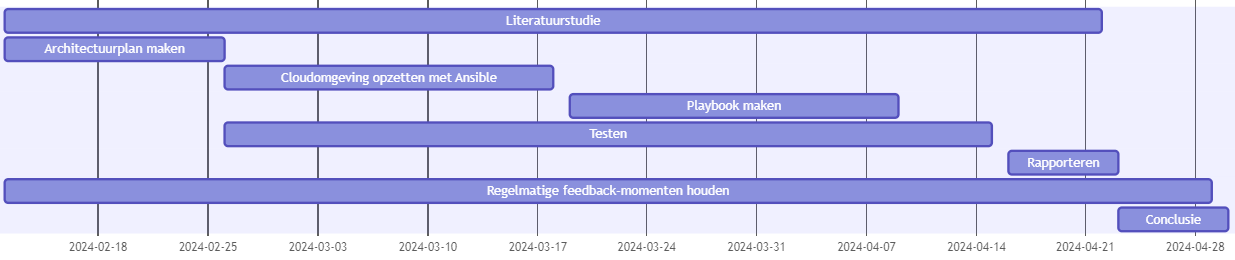
\includegraphics[width=\textwidth]{graphics/gantt.png}
  \caption{Gantt chart}
  \label{fig:gantt}
\end{figure}

%---------- Verwachte resultaten ----------------------------------------------
\section{Verwacht resultaat, conclusie}%
\label{sec:verwachte_resultaten}

De te verwachten resultaten zijn dat dit onderzoek realistisch is en zal bijdragen aan de zoektocht van Aware. Het Proof of Concept is slechts een 
simplistische simulatie van hoe het er aan de werkelijkheid aan toe zou gaan. Het moet bewijzen dat het een mogelijke oplossing is 
voor het probleem en het hoeft daarom niet het finale product zijn.

\section{Discussie, conclusie}
\label{sec:Discussie-conclusie}
Om te bepalen of het Proof of Concept waardig is, wordt het vergeleken met de huidige strategie binnen Aware, waarbij klanten handmatig worden 
opgezet. Dit vergelijkingsproces is essentieel om verschillende aspecten grondig te evalueren, waaronder schaalbaarheid, tijd en 
gebruiksgemak. Door deze factoren te onderzoeken en te analyseren, kan er een dieper inzicht worden verkregen in de potentiële voordelen en mogelijke 
beperkingen van het voorgestelde concept.



\printbibliography[heading=bibintoc]

\end{document}